Черная кривая -- снятый сигнал, $\cmark$ насыщающий пучок.
Красная кривая -- снятый сигнал, $\xmark$ насыщающий пучок.




\begin{figure}[h!]
    \centering
    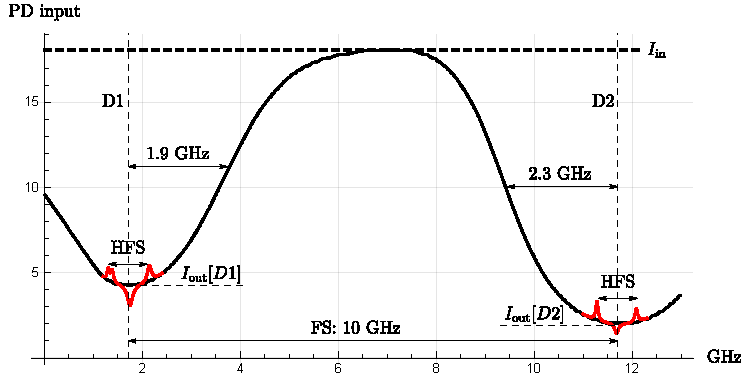
\includegraphics[width=1\textwidth]{D:\\Kami\\git_folder\\notes_5sem\\rqc\\data_processing_1\\exp_D12_v2.pdf}
    \caption{Полученное уширение линий для D1 и D2}
    \label{fig:expD12}
\end{figure}

